\documentclass[]{article}
\usepackage[margin=1in]{geometry} % Sets all margins to 1 inch
\usepackage{amsmath}
\usepackage{tikz}
\usetikzlibrary{
	decorations.pathmorphing,
	decorations.markings,
	positioning,
	arrows.meta,
	calc,
	shapes.geometric
}


\usepackage{tabularx} % Add this to your preamble (before \begin{document})
\usepackage{booktabs} % Optional: For professional looking lines (\toprule, \midrule, \bottomrule)


%opening
\title{PID Controller}
\author{Gaurav Upreti}

\begin{document}

\maketitle

\section{Introduction}
A \textbf{controller} is the ``brain'' of an automated system. It regulates a piece of hardware by repeating the same three steps again and again:
\begin{enumerate}
	\item \textbf{Measure:} use a sensor to read the variable we care about (a speed, a position, an angle, a temperature).
	\item \textbf{Compare:} calculate the \textbf{error}, the difference between where we want to be (the target) and where we are right now:
	\begin{equation}
		\text{error} = \text{target} - \text{actual value}.
	\end{equation}
	\item \textbf{Act:} adjust the machinery in proportion to that error, so that the gap shrinks.
\end{enumerate}
Because this cycle repeats many times per second, the gap is reduced a little at every step until the actual value reaches the target.

\subsection{A daily-life example: running to a spot in a field}
Imagine you are running across a field to reach a marked spot and stop exactly on it. You are acting as a controller:
\begin{itemize}
	\item \textbf{Sensor:} your eyes, which tell you how far away the spot is.
	\item \textbf{Error:} the remaining distance to the spot.
	\item \textbf{Actuator:} your legs, which set your running speed.
\end{itemize}
Every few strides you look up and check how far you still are. When the spot is far away (large error), you run fast. As you get closer (smaller error), you slow down. When the error is almost zero, you are nearly walking, and you stop right on the spot. If you ran at full speed the whole way, you would overshoot, which is exactly what happens to a machine when its controller reacts too strongly.

\subsection{The feedback loop}
Figure~\ref{fig:general_control} shows the cycle as a loop. Information flows from the target, through the controller and the machine, and returns through the sensor to be compared with the target again. This return path is called \textbf{feedback}.


\begin{figure}[ht]
	\centering
	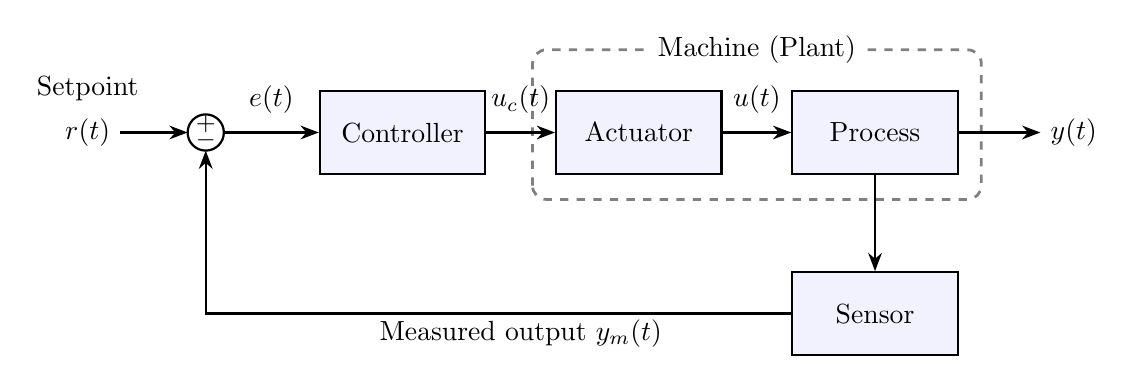
\begin{tikzpicture}[
		>=Stealth,
		thick,
		block/.style={
			draw,
			rectangle,
			minimum width=2.1cm,
			minimum height=1.05cm,
			align=center,
			fill=blue!5
		}
		]
		
		% Setpoint
		\node at (0,0) (ref) {$r(t)$};
		\node at (0,0.55) {Setpoint};
		
		% Summing junction
		\draw (1.5,0) circle (0.23);
		\node at (1.5,0.105) {\small $+$};
		\node at (1.5,-0.105) {\small $-$};
		
		% Controller
		\node[block] (controller) at (4,0)
		{Controller};
		
		% Plant enclosure
		\draw[
		dashed,
		rounded corners=5pt,
		gray,
		line width=1pt
		]
		(5.65,-0.85) rectangle (11.35,1.05);
		
		\node[fill=white,inner sep=3pt]
		at (8.5,1.05) {Machine (Plant)};
		
		% Actuator
		\node[block] (actuator) at (7,0)
		{Actuator};
		
		% Process
		\node[block] (process) at (10,0)
		{Process};
		
		% Forward path
		\draw[->] (ref) -- (1.27,0);
		
		\draw[->] (1.73,0) --
		node[above=3pt] {$e(t)$}
		(controller.west);
		
		% Controller to actuator
		\draw[->] (controller.east) --
		node[above=3pt] {$u_c(t)$}
		(actuator.west);
		
		% Actuator to process
		\draw[->] (actuator.east) --
		node[above=3pt] {$u(t)$}
		(process.west);
		
		% Process output
		\draw[->] (process.east) -- (12.1,0)
		node[right] {$y(t)$};
		
		% Sensor
		\node[block] (sensor) at (10,-2.3)
		{Sensor};
		
		% Process to sensor
		\draw[->] (process.south) -- (sensor.north);
		
		% Feedback path
		\draw[->] (sensor.west) --
		(1.5,-2.3) --
		(1.5,-0.23);
		
		% Feedback label
		\node at (5.5,-2.55)
		{Measured output $y_m(t)$};
		
	\end{tikzpicture}
	
	\caption{The feedback loop: the target is compared with the sensor reading, the error drives the controller, and the controller drives the machine.}
	\label{fig:general_control}
\end{figure}

\section{PID Formulation}
One type of controller that is widely used in robotics
At every moment the controller measures the \textbf{error}, the gap between the target (setpoint) $r(t)$ and the actual value $y(t)$:
\begin{equation}
	e(t) = r(t) - y(t).
\end{equation}
The controller output $u(t)$ which is the sum of three terms:
\begin{equation} 
	u(t) = \underbrace{K_p\,e(t)}_{\text{P: present}} + \underbrace{K_i \int_{0}^{t} e(\tau)\,d\tau}_{\text{I: past}} + \underbrace{K_d\, \frac{de(t)}{dt}}_{\text{D: future trend}} .
	\label{eq:pid} 
\end{equation}

\begin{table}[h]
	\centering
	\begin{tabular}{lll}
		\hline
		Symbol & Meaning & Role \\
		\hline
		$e(t)$ & error, target minus actual & --- \\
		$u(t)$ & controller output (force) & --- \\
		$K_p$ & proportional gain & reacts to the \emph{present} error \\
		$K_i$ & integral gain  & reacts to the \emph{accumulated past} error \\
		$K_d$ & derivative gain & reacts to \emph{how fast} the error changes \\
		$\tau$ & dummy time variable inside the integral & --- \\
		\hline
	\end{tabular}
	\caption{variables in the PID formulation.}
\end{table}




\paragraph{P (present):} Push in proportion to how far we are from the target. A large error gives a large push. Larger $K_p$ gives a faster response, but too much causes overshoot and oscillation.
\paragraph{I (past):} Add up the error over time. If a small error persists, the integral keeps growing and pushes harder until the error is removed. This is what eliminates the final offset left by P alone.
\paragraph{D (rate of change):} Look at how quickly the error is changing. If the error is shrinking fast, D reduces the push to brake the motion before overshooting. It acts like damping.


\begin{figure}[ht]
	\centering
	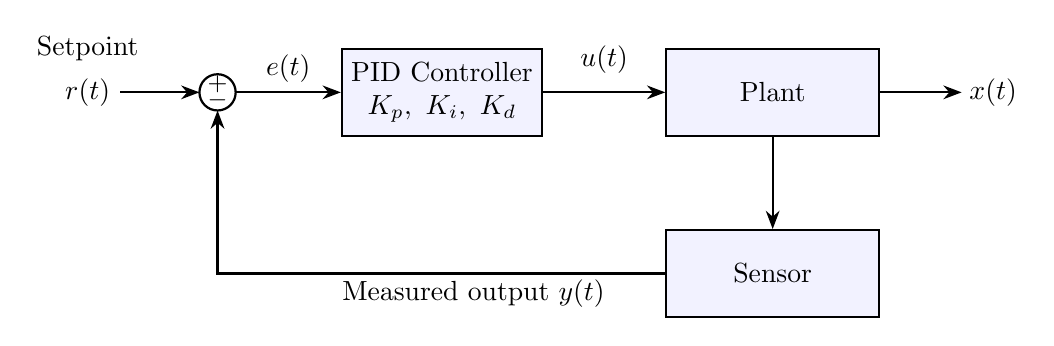
\begin{tikzpicture}[
		>=Stealth,
		thick,
		block/.style={
			draw,
			rectangle,
			minimum width=2.5cm,
			minimum height=1.1cm,
			align=center,
			fill=blue!5
		}
		]
		
		% Setpoint
		\node at (0,0) (ref) {$r(t)$};
		\node at (0,0.55) {Setpoint};
		
		% Summing junction
		\draw (1.65,0) circle (0.23);
		\node at (1.65,0.105) {\small $+$};
		\node at (1.65,-0.105) {\small $-$};
		
		% PID controller
		\node[block] (pid) at (4.5,0)
		{PID Controller\\$K_p,\ K_i,\ K_d$};
		
		% Abstract plant
		\node[block,minimum width=2.7cm] (plant) at (8.7,0)
		{Plant};
		
		% Output
		\node at (11.5,0) (out) {$x(t)$};
		
		% Forward path
		\draw[->] (ref) -- (1.42,0);
		\draw[->] (1.88,0) -- node[above] {$e(t)$} (pid.west);
		
		\draw[->] (pid.east) --
		node[above=3pt] {$u(t)$}
		(plant.west);
		
		\draw[->] (plant.east) -- (11.1,0);
		\node at (10.95,0.25) {};
		
		% Sensor
		\node[block,minimum width=2.7cm] (sensor)
		at (8.7,-2.3) {Sensor};
		
		% Plant to sensor
		\draw[->] (plant.south) -- (sensor.north);
		
		% Feedback loop
		\draw[->] (sensor.west) -- (1.65,-2.3)
		-- (1.65,-0.23);
		
		% Feedback label
		\node at (4.9,-2.55)
		{Measured output $y(t)$};
		
	\end{tikzpicture}
	
	\caption{Closed-loop PID control system.}
	\label{fig:pid_control}
\end{figure}

\subsection{The version a computer runs}
A computer works in small time steps of length $\Delta t$ (the sampling period). At step $k$ the integral becomes a running sum and the derivative becomes a difference:
\begin{align}
	e_k &= r_k - y_k, \\
	I_k &= I_{k-1} + e_k\, \Delta t, \\
	D_k &= \frac{e_k - e_{k-1}}{\Delta t}, \\
	u_k &= K_p\, e_k + K_i\, I_k + K_d\, D_k .
	\label{eq:pid-discrete}
\end{align}
Each cycle the program (1) reads the sensor, (2) computes $e_k$, (3) updates $I_k$ and $D_k$, (4) outputs $u_k$ to the actuator, and (5) waits for the next step.


\section{The Test System}
We control a block of mass $m$ attached to a spring and a damper, similar to a car suspension. The \textbf{block slides horizontally on a frictionless surface}, so gravity acts perpendicular to the motion and does not affect the dynamics. The spring is at its natural length at $x=0$, and a positive force $u$ pushes the block toward positive $x$. The goal is to move the block to $x = r = 1$\,m.

\begin{table}[h]
	\centering
	\begin{tabular}{lll}
		\hline
		Parameter & Value & Unit \\
		\hline
		Mass $m$ & 1 & kg \\
		Damping $c$ & 10 & N$\cdot$s/m \\
		Spring stiffness $k$ & 20 & N/m \\
		Target $r$ & 1 & m \\
		\hline
	\end{tabular}
	\caption{Parameters of the test system.}
\end{table}


\begin{figure}[ht]
	\centering
	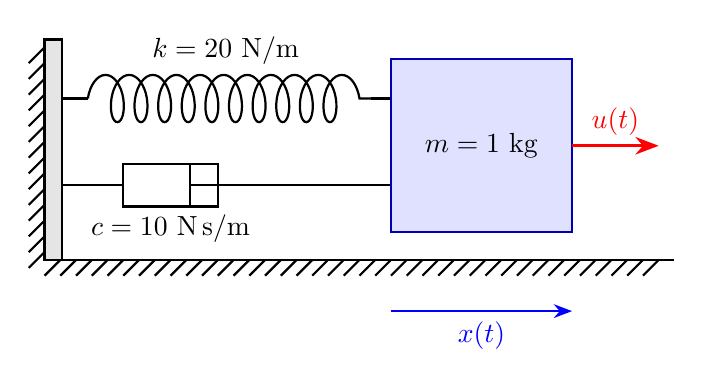
\begin{tikzpicture}[
		>=Stealth,
		thick,
		spring/.style={
			decorate,
			decoration={
				coil,
				aspect=0.5,
				segment length=3mm,
				amplitude=3mm
			}
		}
		]
		
		% Fixed wall
		\draw[fill=gray!20] (0,0) rectangle (0.22,2.8);
		
		\foreach \y in {0.1,0.3,...,2.7}
		\draw (0,\y) -- (-0.2,\y-0.2);
		
		% Ground
		\draw (0,0) -- (8,0);
		
		\foreach \x in {0.2,0.4,...,7.8}
		\draw (\x,0) -- (\x-0.2,-0.2);
		
		% Spring
		\draw (0.22,2.05) -- (0.55,2.05);
		\draw[spring] (0.55,2.05) -- (4.15,2.05);
		\draw (4.15,2.05) -- (4.4,2.05);
		
		\node[above] at (2.3,2.35)
		{$k=20\ \mathrm{N/m}$};
		
		% Damper cylinder
		\draw (0.22,0.95) -- (1.0,0.95);
		\draw (1.0,0.68) rectangle (2.2,1.22);
		
		% Piston
		\draw (1.85,0.68) -- (1.85,1.22);
		
		% Piston rod
		\draw (1.85,0.95) -- (4.4,0.95);
		
		% Damping coefficient
		\node at (1.6,0.40)
		{$c=10\ \mathrm{N\,s/m}$};
		
		% Wider mass block
		\draw[
		fill=blue!12,
		draw=blue!70!black
		]
		(4.4,0.35) rectangle (6.7,2.55);
		
		% Mass label
		\node at (5.55,1.45)
		{$m=1\ \mathrm{kg}$};
		
		% Applied force
		\draw[->,red,very thick]
		(6.7,1.45) -- (7.8,1.45);
		
		\node[above,red] at (7.25,1.45)
		{$u(t)$};
		
		% Displacement
		\draw[->,blue,thick]
		(4.4,-0.65) -- (6.7,-0.65);
		
		\node[below,blue] at (5.55,-0.65)
		{$x(t)$};
		
	\end{tikzpicture}
	
	\caption{Horizontal mass--spring--damper system.}
	\label{fig:mass_spring_damper}
\end{figure}

\subsection{Equation of motion}
Newton's second law (mass times acceleration equals the sum of forces) gives
\begin{equation}
	m\,\ddot{x}(t) + c\,\dot{x}(t) + k\,x(t) = u(t),
	\label{eq:plant}
\end{equation}
that is, with the numbers above,
\begin{equation}
	\ddot{x} = u - 10\,\dot{x} - 20\,x .
\end{equation}
Here $x$ is position (m), $\dot{x}$ is velocity (m/s), $\ddot{x}$ is acceleration (m/s$^2$), $c\dot{x}$ is the damper force and $kx$ is the spring force.

For simulation we write this as two first-order equations with state $(x, v)$, where $v=\dot{x}$:
\begin{equation}
	\dot{x} = v, \qquad
	\dot{v} = \frac{1}{m}\bigl(u - c\,v - k\,x\bigr).
\end{equation}
Taking the Laplace transform with zero initial conditions gives the transfer function
\begin{equation}
	G(s) = \frac{X(s)}{U(s)} = \frac{1}{m s^2 + c s + k} = \frac{1}{s^2 + 10 s + 20}.
\end{equation}

\subsection{Why the spring needs a constant push}
Suppose the block is at rest at the target, so $\dot{x}=0$ and $\ddot{x}=0$. The damper force is zero because there is no motion, and Eq.~\eqref{eq:plant} reduces to
\begin{equation}
	k\,x = u \quad\Longrightarrow\quad u_{\text{hold}} = k\, r = 20 \times 1 = 20\ \text{N}.
\end{equation}
The stretched spring pulls the block back with 20N, so something must push forward with exactly 20N to hold it at 1m. Without this constant force the block drifts back to $x=0$. This is the key fact behind the steady-state error of P-only control (Section~5) and the role of the integral term.

\subsection{Open-loop behaviour}
The \emph{DC gain} (the final position per newton of constant force) is $G(0) = 1/k = 0.05$m/N. The natural frequency and damping ratio are
\begin{equation}
	\omega_n = \sqrt{k/m} = \sqrt{20} \approx 4.47\ \text{rad/s}, \qquad
	\zeta = \frac{c}{2\sqrt{km}} = \frac{10}{2\sqrt{20}} \approx 1.12 .
\end{equation}
Since $\zeta > 1$ the system is overdamped: left alone it moves smoothly to its final value without oscillating. Its poles are real, at $s = -5 \pm \sqrt{5} \approx -2.76$ and $-7.24$s$^{-1}$. Any oscillation or overshoot seen later is therefore caused by the controller, not by the plant.


\section{Results}

\subsection{How to Judge a Result}

A controller is judged on the \textbf{step response}: the target jumps from 0 to $r = 1$\,m at $t=0$ and we watch how $y(t)$ reacts. Four numbers describe the response (Figure~\ref{fig:metrics}).

\begin{enumerate}
	\item \textbf{Rise time $T_r$} (speed): the time to go from 10\% to 90\% of the target, i.e.\ from 0.1\,m to 0.9\,m. Smaller is faster. If $y$ never reaches 0.9\,m we write ``never''.
	\item \textbf{Overshoot $M_p$} (how far past the target):
	\begin{equation}
		M_p = \max\!\left(0,\ \frac{y_{\max} - r}{r}\right) \times 100\%.
	\end{equation}
	\item \textbf{Settling time $T_s$} (how long until calm): the last time the output is outside the $\pm 2\%$ band around the target ($|e| > 0.02$\,m). After $T_s$ the response stays inside the band.
	\item \textbf{Steady-state error $e_{ss}$} (where it finally stops): the error at the end of the run,
	\begin{equation}
		e_{ss} = r - y(t_{\text{end}}).
	\end{equation}
\end{enumerate}

\begin{figure}[h]
	\centering
	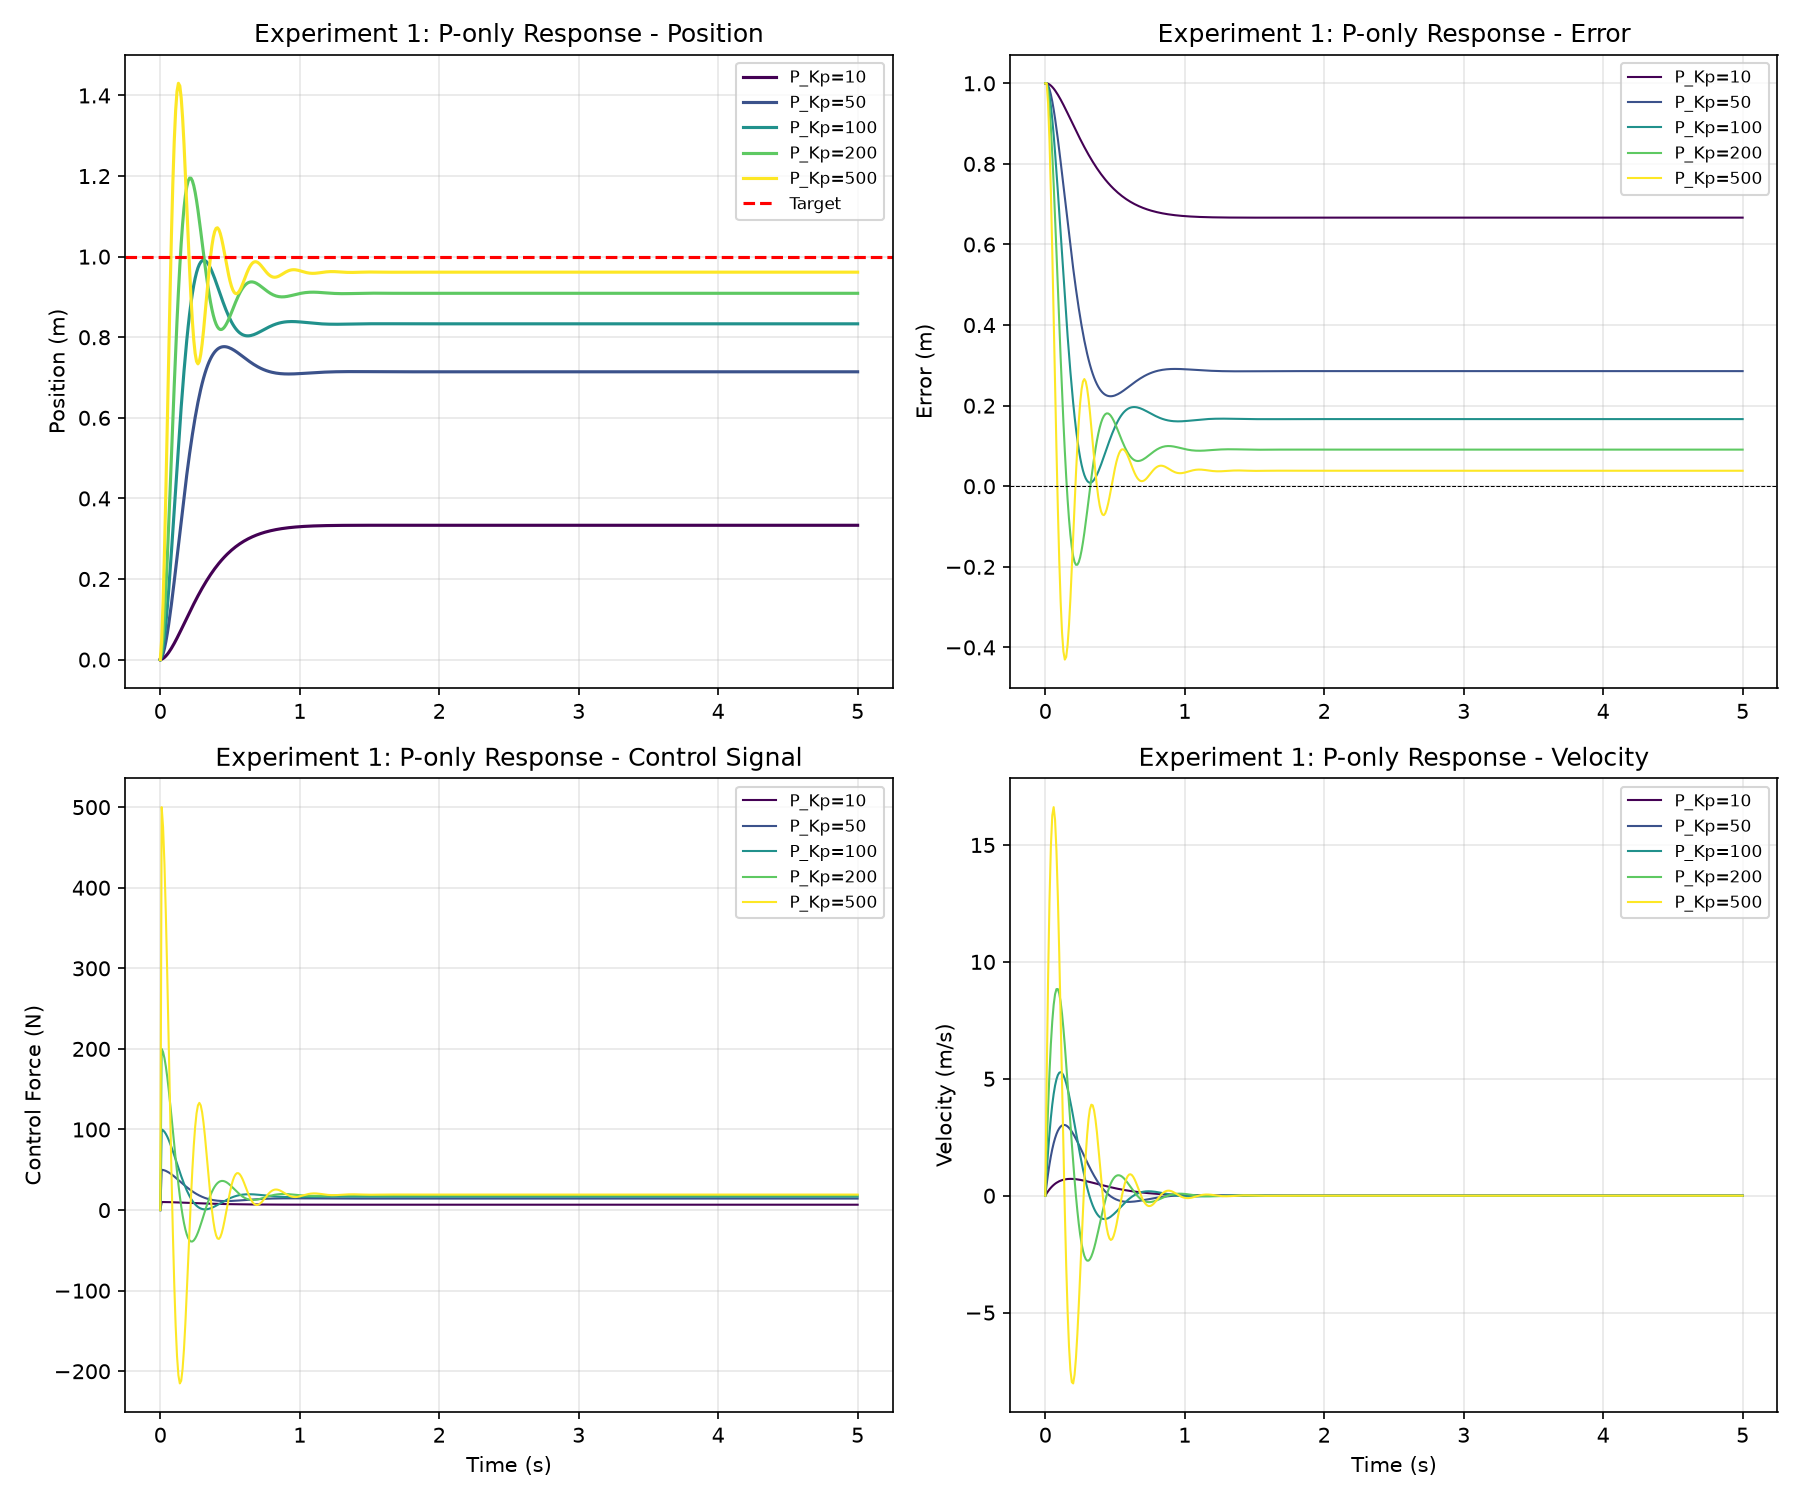
\includegraphics[width=0.85\linewidth]{experiment_plots/exp1_p_only.png}
	\caption{Step response of a PID-controlled block with the four measures marked: rise time (10\%$\to$90\%), overshoot, settling time ($\pm2\%$ band) and steady-state error.}
	\label{fig:metrics}
\end{figure}

All measures are taken relative to the \emph{target}, not relative to where the output happens to settle. This matters for a P-only controller, which settles below the target: it has a large steady-state error even if its overshoot is 0\%.

%--------------------------------------------------------------------

\subsection{Each Part Alone}

All runs use the test system of Section~3 with a step to $r=1$\,m, a time step of 1\,ms (the controller runs at the same step) and a 5\,s simulation.

\begin{figure}[h]
	\centering
	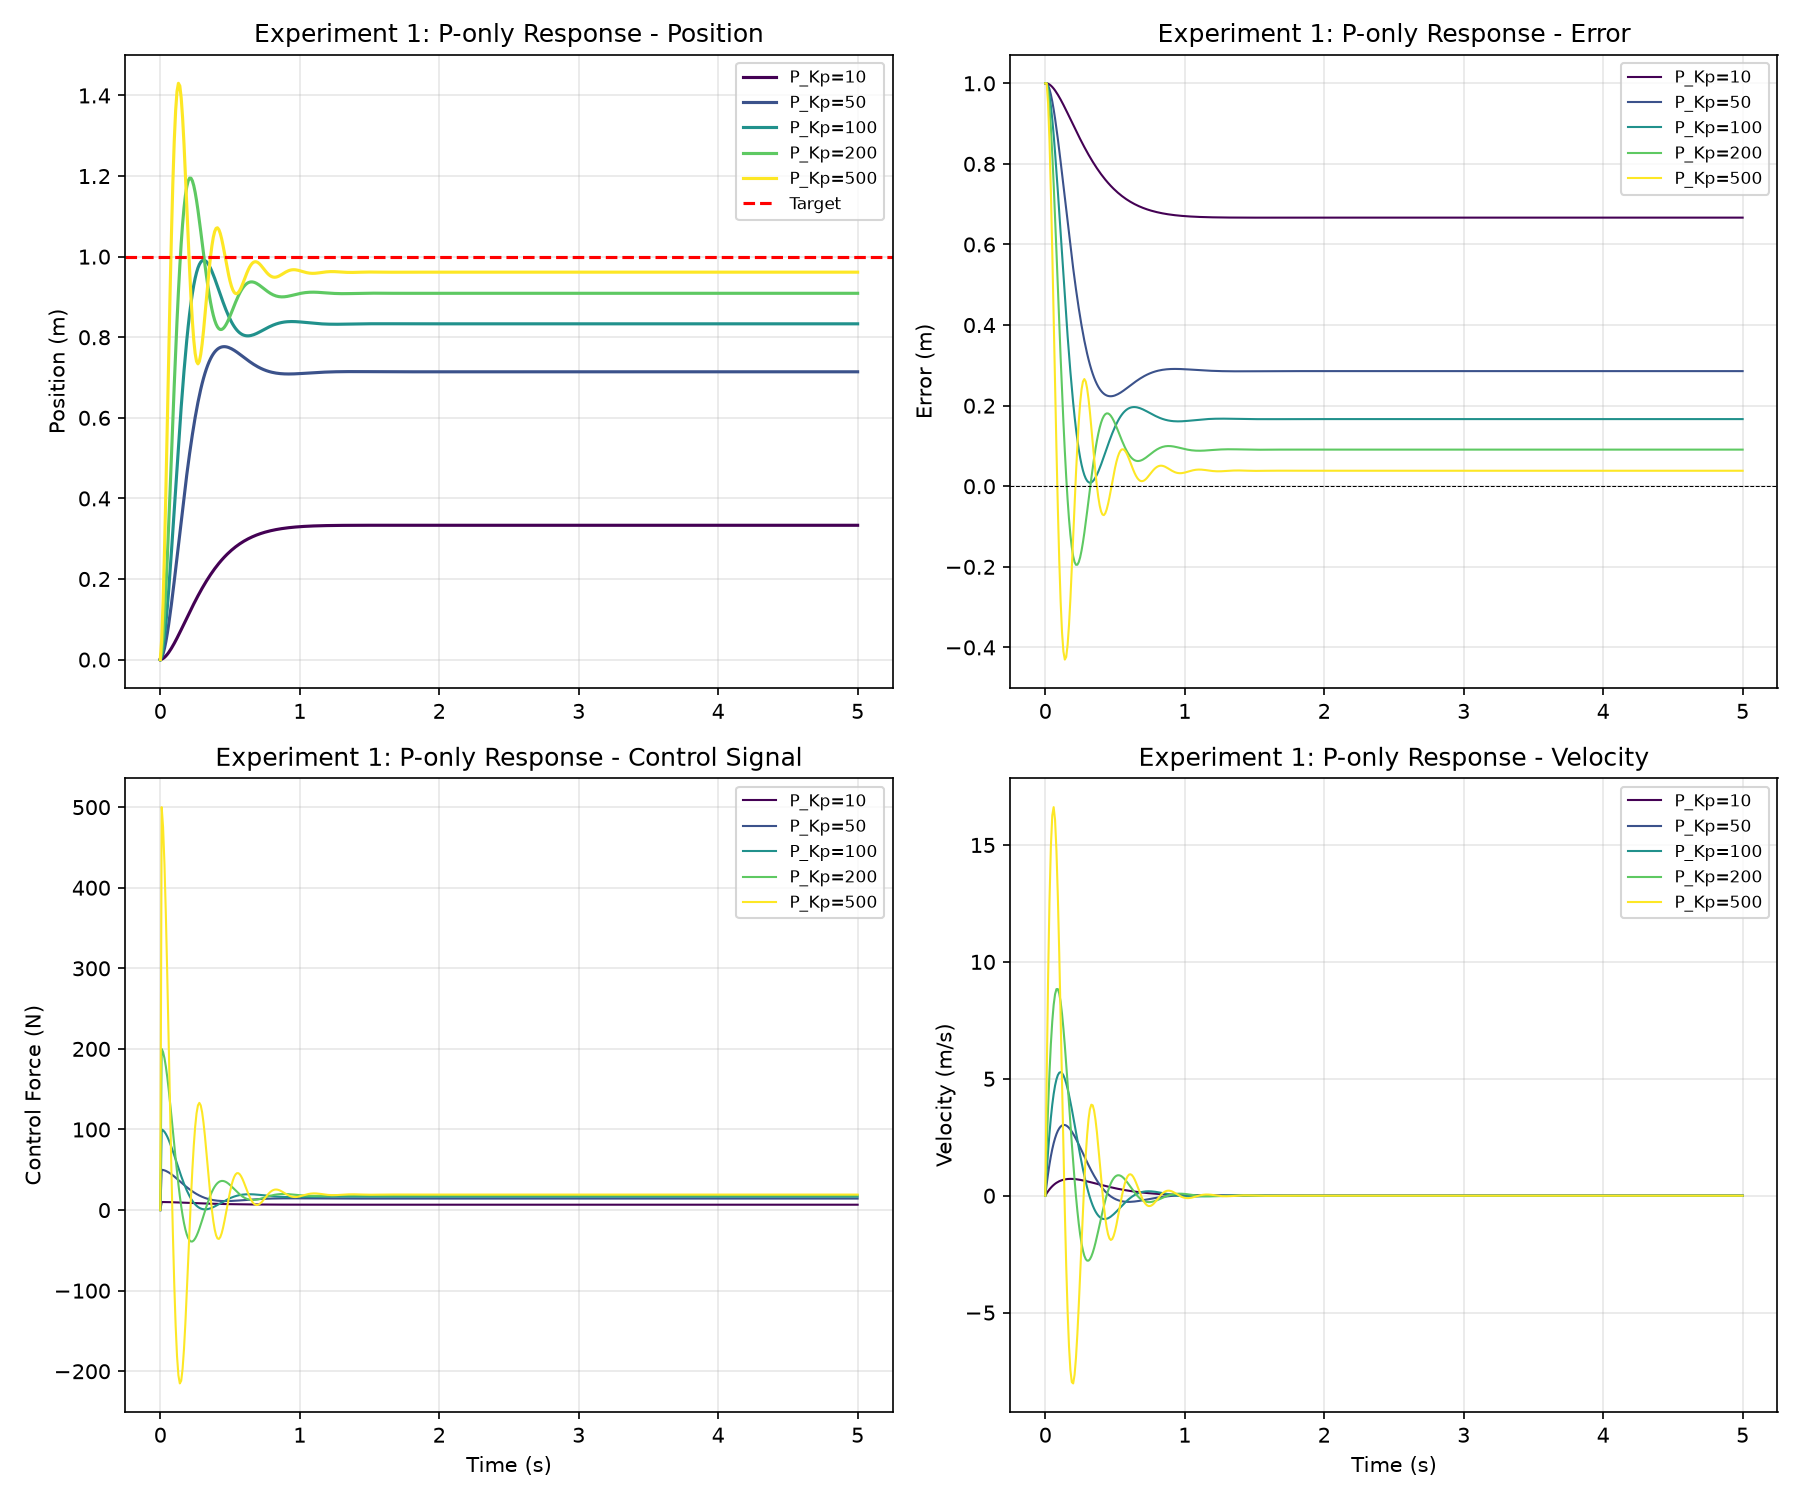
\includegraphics[width=0.85\linewidth]{experiment_plots/exp1_p_only.png}
	\caption{P-only step responses for $K_p = 10, 50, 100, 200, 500$\,N/m. Every curve stops below the 1\,m target, and larger $K_p$ gets closer but oscillates more.}
\end{figure}
\subsubsection{P only}

Using $u = K_p e$ in the plant equation $\ddot{x} = u - 10\dot{x} - 20x$ with the block at rest ($\dot{x}=\ddot{x}=0$):
\begin{equation}
	K_p (r - x_{ss}) = 20\,x_{ss}
	\;\Longrightarrow\;
	x_{ss} = \frac{K_p}{20 + K_p}\, r,
	\qquad
	e_{ss} = \frac{20}{20 + K_p}\, r .
	\label{eq:pss}
\end{equation}
\textbf{Why P alone stops short:} at the target the spring needs 20\,N. A P controller only pushes when there is an error, so it needs an error of $20/K_p$ to produce that force. Zero error would mean zero push, and the spring would pull the block back. The error can be made smaller with a larger $K_p$ but never zero.

\begin{table}[h]
	\centering
	\begin{tabular}{@{}rrrrr@{}}
		\toprule
		$K_p$ (N/m) & Predicted $x_{ss}$ (m) & Predicted $e_{ss}$ (m) & Measured $e_{ss}$ (m) & Overshoot (\%) \\
		\midrule
		10  & 0.333 & 0.6667 & 0.6667 & 0 \\
		50  & 0.714 & 0.2857 & 0.2857 & 0 \\
		100 & 0.833 & 0.1667 & 0.1667 & 0 \\
		200 & 0.909 & 0.0909 & 0.0909 & 20.3 \\
		500 & 0.962 & 0.0385 & 0.0385 & 43.5 \\
		\bottomrule
	\end{tabular}
	\caption{P-only control: prediction from Eq.~\eqref{eq:pss} versus simulation.}
	\label{tab:ponly}
\end{table}

The measured errors in Table~\ref{tab:ponly} agree with the formula to four decimals. The overshoot is relative to the target, so the 200 and 500 curves cross 1\,m and swing back. For $K_p \le 100$ the curve stays below 1\,m, but it can still oscillate (see Section 5.3).

\subsubsection{Adding I}

The integral term accumulates the error, $u = K_p e + K_i\int e\,dt$. In steady state $e$ is constant and the integral keeps growing as long as $e \neq 0$, so the only way to stop is $e = 0$. Then the integral term itself must hold the spring force:
\begin{equation}
	K_i \int_0^{\infty} e\, d\tau = k\,r = 20\ \text{N}.
\end{equation}
With $K_p = 100$ and $K_i = 50$ the error at $t=5$\,s has fallen from 0.1667\,m (P only) to 0.0164\,m, and keeps shrinking toward zero. The price is a small overshoot of 5.7\% and a slow tail, because the integral builds up gradually.

\subsubsection{Adding D}

With P only, the closed loop is $s^2 + 10s + (20+K_p)$ and its damping ratio is
\begin{equation}
	\zeta_P = \frac{10}{2\sqrt{20 + K_p}} .
\end{equation}
The derivative term is a force proportional to velocity, so it adds to the damper: $s^2 + (10+K_d)s + (20+K_p)$, and
\begin{equation}
	\zeta_{PD} = \frac{10 + K_d}{2\sqrt{20 + K_p}} .
\end{equation}
The oscillation overshoot (relative to the final value) is $\exp\!\bigl(-\pi\zeta/\sqrt{1-\zeta^2}\bigr)$. For $K_p = 100$:
\begin{center}
	\begin{tabular}{@{}lccc@{}}
		\toprule
		& $\zeta$ & Predicted overshoot of oscillation \\
		\midrule
		P ($K_d=0$)   & 0.456 & 20.0\% of $x_{ss}$ \\
		PD ($K_d=10$) & 0.913 & 0.1\% of $x_{ss}$ \\
		\bottomrule
	\end{tabular}
\end{center}
So $K_d = 10$ doubles the damping ratio and removes almost all the bouncing. $K_d = 2\sqrt{20+K_p} - 10 \approx 11.9$ would make it exactly critically damped ($\zeta=1$). D does \emph{not} change the steady-state error, which stays at 0.1667\,m, because $\dot{e}=0$ at rest.

%--------------------------------------------------------------------

\subsection{All Together}

Figure~\ref{fig:all} compares P, PI, PD and PID on the same step, and Table~\ref{tab:all} gives the four measures of Section~4.

\begin{figure}[h]
	\centering
	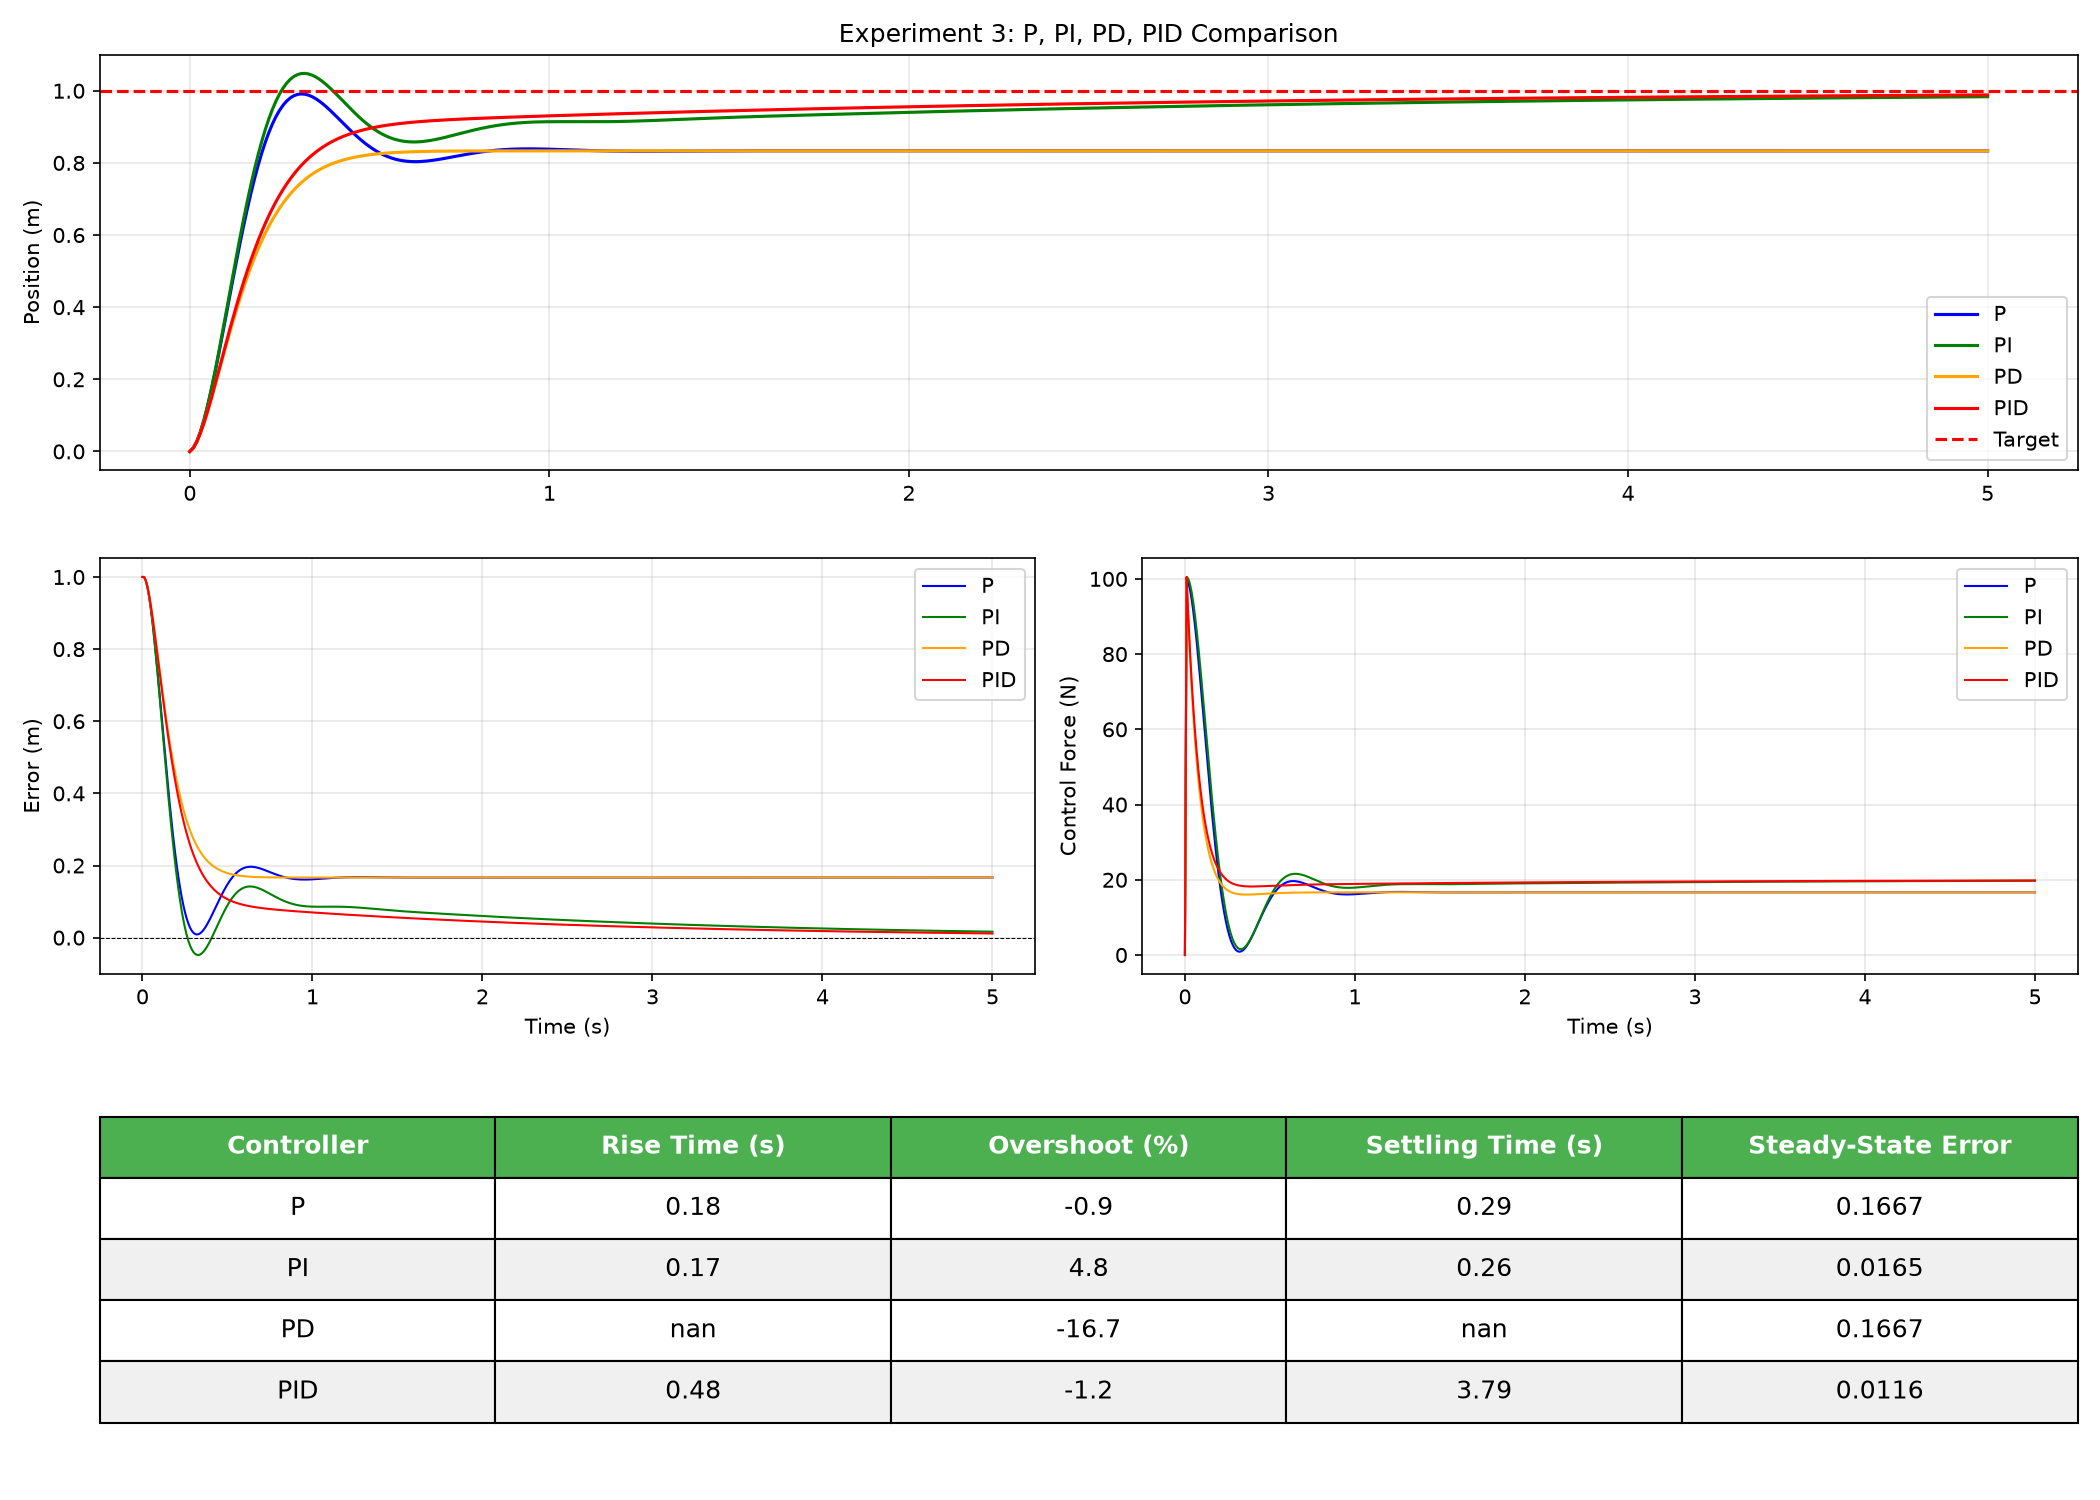
\includegraphics[width=0.9\linewidth]{experiment_plots/exp3_comparison.png}
	\caption{Step responses of P, PI, PD and PID with $K_p=100$, $K_i=50$, $K_d=10$.}
	\label{fig:all}
\end{figure}

\begin{table}[h]
	\centering
	\begin{tabular}{@{}lrrrr@{}}
		\toprule
		Controller & Rise time (s) & Overshoot (\%) & Settling time (s) & $e_{ss}$ (m) \\
		\midrule
		P   ($K_p=100$)                    & 0.18  & 0.0 & never & 0.1667 \\
		PI  ($K_i=50$)                      & 0.17  & 5.7 & 4.54 & 0.0164 \\
		PD  ($K_d=10$)                      & never & 0.0 & never & 0.1667 \\
		PID ($K_p=100,\,K_i=50,\,K_d=10$)   & 0.45  & 0.0 & 3.78 & 0.0115 \\
		\midrule
		Final PID (chosen gains)            & \textbf{[fill]} & \textbf{[fill]} & \textbf{[fill]} & \textbf{[fill]} \\
		\bottomrule
	\end{tabular}
	\caption{Four measures for each controller type (5\,s run, 1\,ms step).}
	\label{tab:all}
\end{table}

\paragraph{What each part contributed.}
P gives the fast initial move but leaves a 16.7\% offset. PI removes the offset ($e_{ss}$ 0.1667\,m $\to$ 0.0164\,m) at the cost of 5.7\% overshoot. PD does not remove the offset but damps the oscillation. PID has no overshoot and the smallest final error, but it is slower to rise because the D term brakes the initial motion.

\paragraph{Final gains.}
We choose $K_p = [\ldots]$, $K_i = [\ldots]$, $K_d = [\ldots]$, giving overshoot of [\ldots]\%, settling time of [\ldots]\,s and $e_{ss}<$ [\ldots]\,mm. Reasoning: $K_p$ sets the speed, and we increased it until the rise time was about [\ldots]\,s while the 30\,N limit of Section~7 is respected. $K_d$ was set close to the critical-damping value of Section~5.3 to prevent bouncing, and $K_i$ is as large as possible without raising overshoot above [\ldots]\%, because a larger $K_i$ also makes windup worse (Section~7a).

\section{Real-world Problems}

The ideal PID of Section~2 assumes a perfect actuator, a perfect sensor and instant computation. Real machines break all three assumptions. This section shows four resulting problems on the test system of Section~3 (1\,m step) and fixes each one.

%--------------------------------------------------------------------
\subsection{(a) Integral windup}

\paragraph{The problem.}
Every real actuator has a limit: a motor can spin only up to a maximum rpm, a servo can turn only to a maximum angle, and a quadcopter propeller can give only a maximum thrust. Here the actuator can push at most $\pm 30$\,N. The controller does not know this. While the block is far from the target the controller asks for more than 30\,N, the actuator delivers only 30\,N, so the error stays large and the integral term keeps accumulating:
\begin{equation}
	I(t) = \int_0^t e(\tau)\,d\tau \ \text{ keeps growing while } u_{\text{raw}} > 30\,\text{N}.
\end{equation}
Nothing looks wrong at that moment, because the output is clipped anyway. The damage appears \emph{later}. When the block reaches the target the error is zero, but the integral term $K_i I$ is still huge. In our run it reaches about 57\,N, while only 20\,N is needed to hold the spring (Section~3). The excess force keeps pushing the block past the target. The integral can only decrease when the error is \emph{negative}, so the block must first overshoot and spend time on the wrong side of the target until the accumulated area has been cancelled out:
\begin{equation}
	\int e\,dt \ \text{must reach}\ -\frac{57 - 20}{K_i} = -0.185\ \text{m$\cdot$s}.
\end{equation}
This unwinding takes time, and that delay is the lag seen in the graph.

\begin{figure}[h]
	\centering
	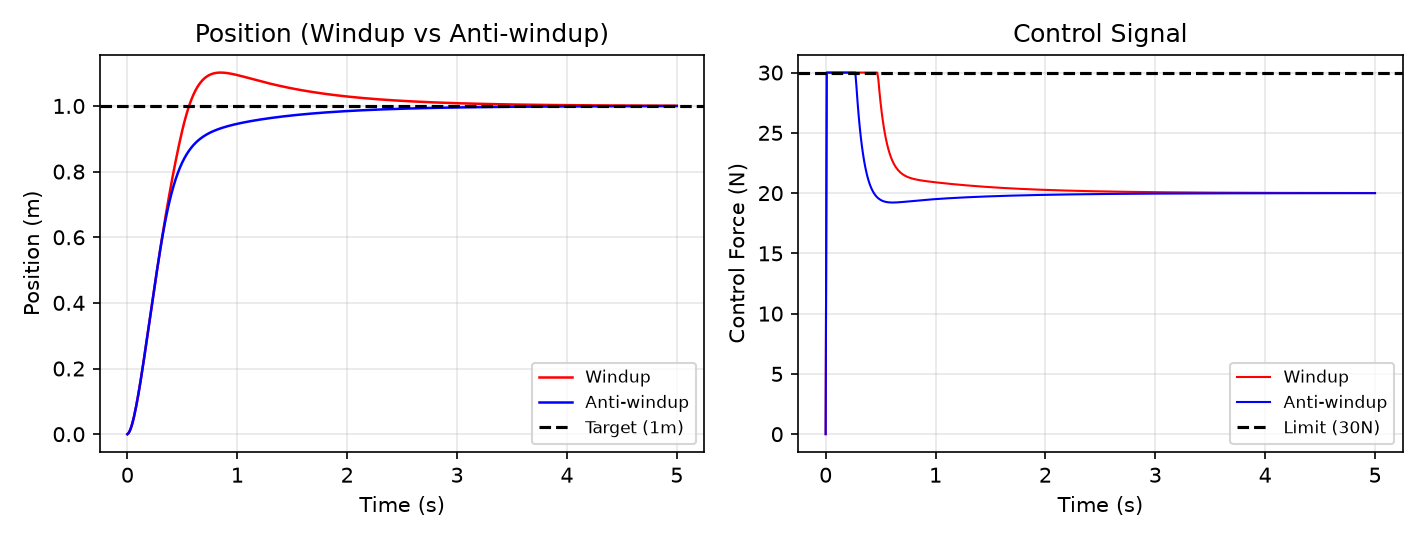
\includegraphics[width=0.9\linewidth]{experiment_plots/exp4a_windup.png}
	\caption{Windup ($K_p=40$, $K_i=200$, $K_d=0$, force limit $\pm30$\,N): position, force and integral term. The integral grows during saturation and the block overshoots the 1\,m target to 1.353\,m (35.3\%).}
\end{figure}

\paragraph{The fix: clamping (conditional integration).}
The cheapest fix is to stop the integral from growing while the actuator is saturated and the error would push it further into saturation:
\begin{equation}
	I_k =
	\begin{cases}
		I_{k-1} & \text{if } u_{\text{raw},k} > u_{\max} \text{ and } e_k > 0,\ \text{or } u_{\text{raw},k} < u_{\min} \text{ and } e_k < 0,\\[2pt]
		I_{k-1} + e_k\,\Delta t & \text{otherwise.}
	\end{cases}
\end{equation}
Other methods exist (back-calculation, integral limits), but this one needs no extra tuning parameter.

\begin{figure}[b]
	\centering
	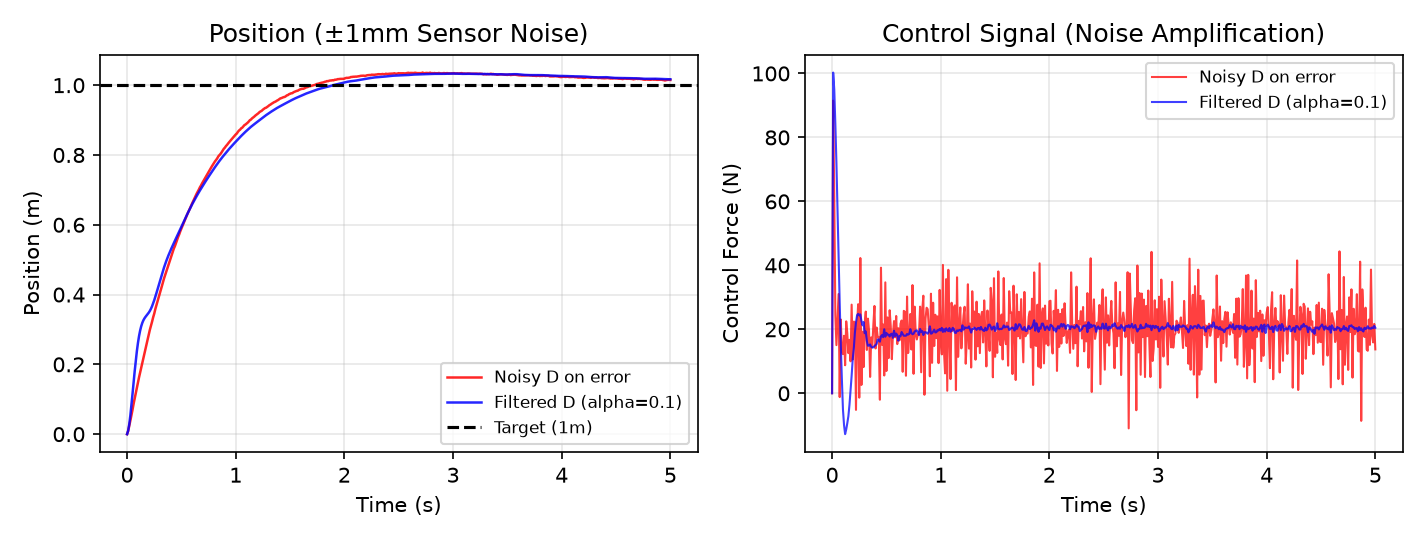
\includegraphics[width=0.9\linewidth]{experiment_plots/exp4b_noise.png}
	\caption{Same gains with clamping. The integral stops growing while the force is at 30\,N, and the overshoot falls from 35.3\% to 7.1\% (peak 1.353\,m $\to$ 1.071\,m). The peak integral force falls from 57\,N to 23\,N.}
\end{figure}

%--------------------------------------------------------------------
\subsection{(b) Sensor noise and the derivative term}

\paragraph{The problem.}
The derivative term measures \emph{how fast the error changes}, i.e.\ the difference between two readings divided by a small time step. Real sensors always add noise, and dividing a tiny difference by a tiny $\Delta t$ makes it large. For a sine wave $A\sin(\omega t)$ the derivative has amplitude $A\omega$, so
\begin{equation}
	\left|\frac{d}{dt}\bigl(A\sin\omega t\bigr)\right|_{\max} = A\,\omega .
\end{equation}
The derivative depends on the \emph{frequency} as well as on the amplitude. A 1\,mm noise component at 50\,Hz ($\omega = 314$\,rad/s) has a slope of $0.001 \times 314 = 0.31$\,m/s. A real motion of $A = 0.1$\,m at only 0.5\,Hz ($\omega = 3.14$\,rad/s) produces the same slope. At 500\,Hz the 1\,mm noise already gives 3.1\,m/s. So noise that is invisible on the position graph becomes large in the D term, and the force becomes jumpy.

For white noise of standard deviation $\sigma$ with samples $\Delta t$ apart, the difference of two samples has a standard deviation $\sqrt{2}\sigma$. The derivative noise is therefore
\begin{equation}
	\sigma_{\dot e} = \frac{\sqrt{2}\,\sigma}{\Delta t}
	= \frac{1.41 \times 0.001}{0.01} = 0.14\ \text{m/s}.
\end{equation}
Multiplied by $K_d = 10$ this is a force noise of about 1.4\,N, which is what the simulation shows (1.59\,N standard deviation, Table~\ref{tab:noise}). A real motor would be shaken by this at every sample.

\paragraph{The fix: low-pass filter on the derivative.}
We pass the derivative through a first-order low-pass filter, which lets slow changes through and suppresses fast ones:
\begin{equation}
	D_k^{\text{filt}} = \alpha\, D_k + (1-\alpha)\, D_{k-1}^{\text{filt}}, \qquad 0 < \alpha \le 1 ,
\end{equation}
with $\alpha = 0.1$ and $\Delta t = 0.01$\,s, which is a filter time constant of $\tau = \Delta t(1-\alpha)/\alpha = 0.09$\,s (cutoff $\approx 1.8$\,Hz). The cost is a slightly delayed D action, since smaller $\alpha$ means more smoothing and more lag.

\begin{table}[h]
	\centering
	\begin{tabular}{@{}lrr@{}}
		\toprule
		& $K_d = 10$ & $K_d = 50$ \\
		\midrule
		Standard deviation of $u$, unfiltered (N) & 1.59 & 9.50 \\
		Standard deviation of $u$, filtered (N)   & 0.24 & 0.66 \\
		\bottomrule
	\end{tabular}
	\caption{Force noise in steady state with $\pm1$\,mm sensor noise ($K_p=100$, $K_i=50$, $\Delta t=0.01$\,s, fixed random seed). The filter cuts the noise by 85--93\%.}
	\label{tab:noise}
\end{table}


%--------------------------------------------------------------------
\subsection{(c) Derivative kick}

\paragraph{The problem.}
If the target jumps suddenly, the error jumps by the same amount in a single time step, and the derivative of a jump is huge:
\begin{equation}
	D = K_d\,\frac{e_k - e_{k-1}}{\Delta t} \approx K_d\,\frac{\Delta r}{\Delta t}
	= 10 \times \frac{1\,\text{m}}{0.01\,\text{s}} = 1000\ \text{N}.
\end{equation}
Together with the P term ($K_p\Delta r = 100$\,N) the force spikes to about 1100\,N for one step. This is the \emph{derivative kick}. It would saturate any real actuator and can damage hardware, and the spike lasts only one sample, so it does nothing useful for the motion. The same happens when the sensor reading jumps suddenly.

\paragraph{The fix: differentiate the measurement, not the error.}
Since $e = r - y$, we have $\dot e = \dot r - \dot y$. The target $r$ is constant between steps, so $\dot r = 0$ except at the instant of the jump, and we can drop it:
\begin{equation}
	D = -K_d\,\frac{y_k - y_{k-1}}{\Delta t}.
\end{equation}
The result is the same during normal motion, but the target jump no longer enters the derivative. The measurement $y$ is a physical position of a block with mass, so it cannot jump.

\begin{figure}[h]
	\centering
	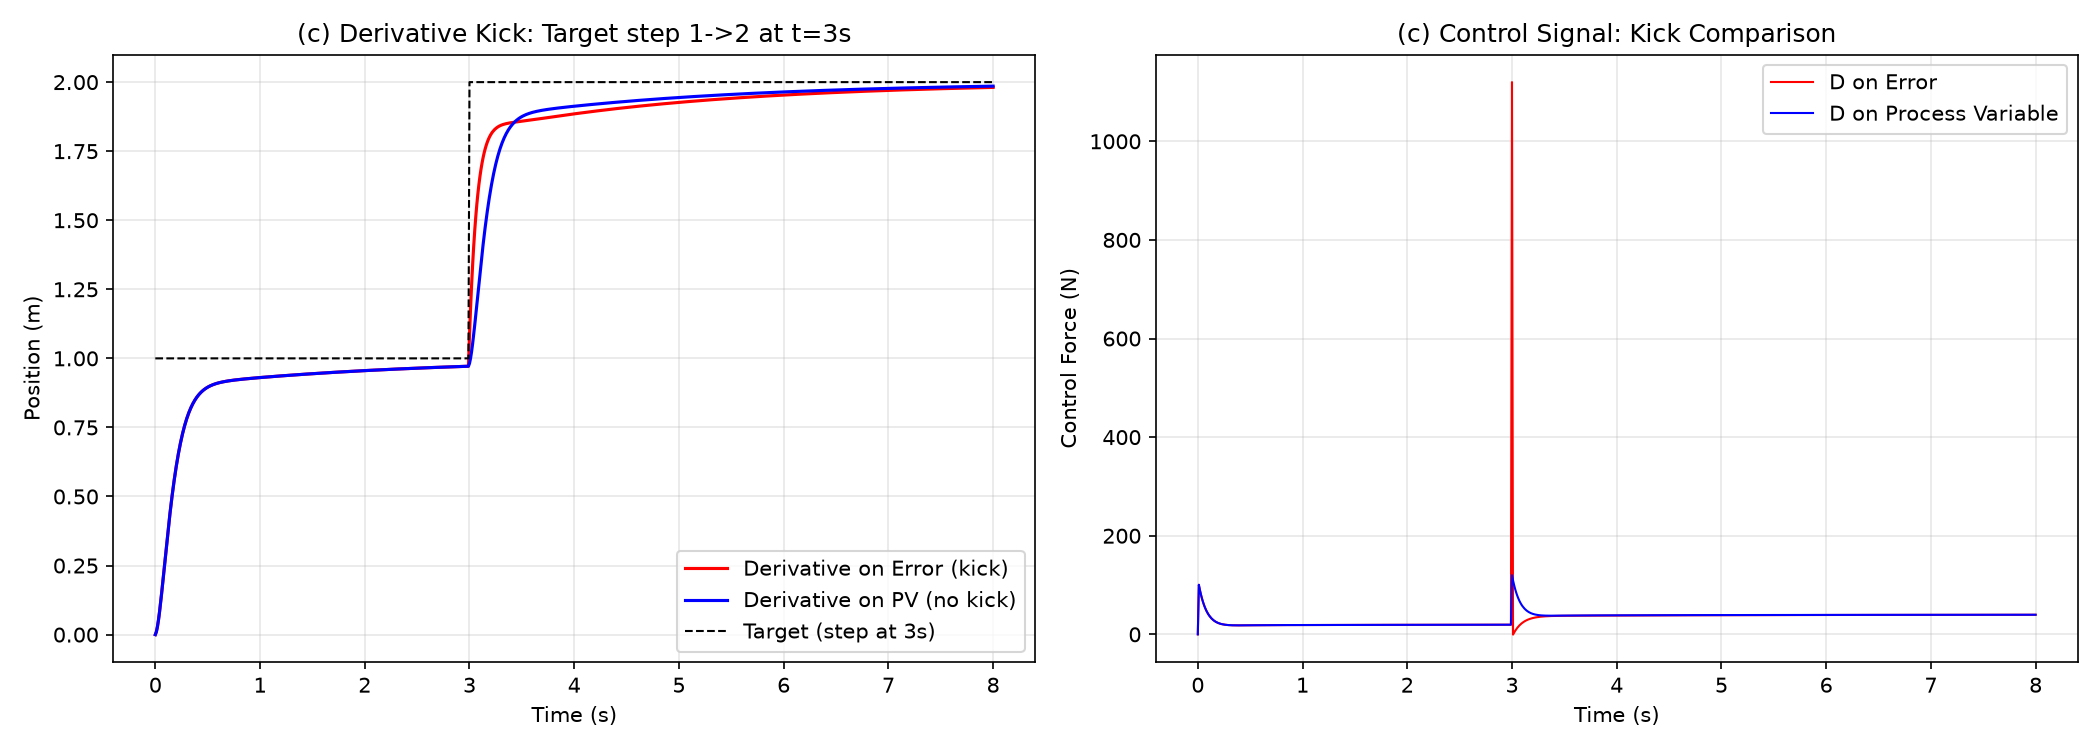
\includegraphics[width=0.9\linewidth]{experiment_plots/exp4c_kick.png}
	\caption{Target stepped from 1\,m to 2\,m at $t=3$\,s ($K_p=100$, $K_i=50$, $K_d=10$, $\Delta t=0.01$\,s). Left: D on error, with a force spike of about 1100\,N. Right: D on measurement. The spike falls to about 120\,N, which is only the P jump ($K_p\Delta r=100$\,N) plus the existing holding force.}
\end{figure}

The remaining 100\,N jump comes from the P term. It can be removed with setpoint weighting or a ramped setpoint, or limited by the 30\,N actuator clamp.

%--------------------------------------------------------------------
\subsection{(d) Slow computer update}

\paragraph{The problem.}
A digital controller does not act continuously. It reads the sensor, computes $u$ and then \emph{holds} that value (zero-order hold) until the next update $T_s$ seconds later. During that time the controller is blind: the block keeps moving while the force stays fixed. This acts like a delay of about $T_s/2$, and delay removes the damping that D and P rely on. The slower the update, the worse the response.

To separate this effect from numerical errors, the plant is always simulated with a fixed 1\,ms step and the controller updates only every $T_s$. The integral and derivative use $T_s$ as their time step.

\begin{table}[h]
	\centering
	\begin{tabular}{@{}rrr@{}}
		\toprule
		Update time $T_s$ & Overshoot (\%) & Result \\
		\midrule
		1\,ms   & 0.0 & settles in 3.78\,s \\
		10\,ms  & 0.0 & settles in 3.77\,s \\
		50\,ms  & 0.0 & settles in 3.74\,s \\
		100\,ms & 0.0 & settles in 3.70\,s \\
		150\,ms & 11.4 & oscillates, settles in 4.01\,s \\
		200\,ms & 41.6 & still oscillating at 5\,s \\
		250\,ms & 117.5 & large oscillation, still growing slowly \\
		300\,ms & --- & unstable (output diverges) \\
		\bottomrule
	\end{tabular}
	\caption{Effect of the controller update time ($K_p=100$, $K_i=50$, $K_d=10$).}
	\label{tab:ts}
\end{table}

\begin{figure}[h]
	\centering
	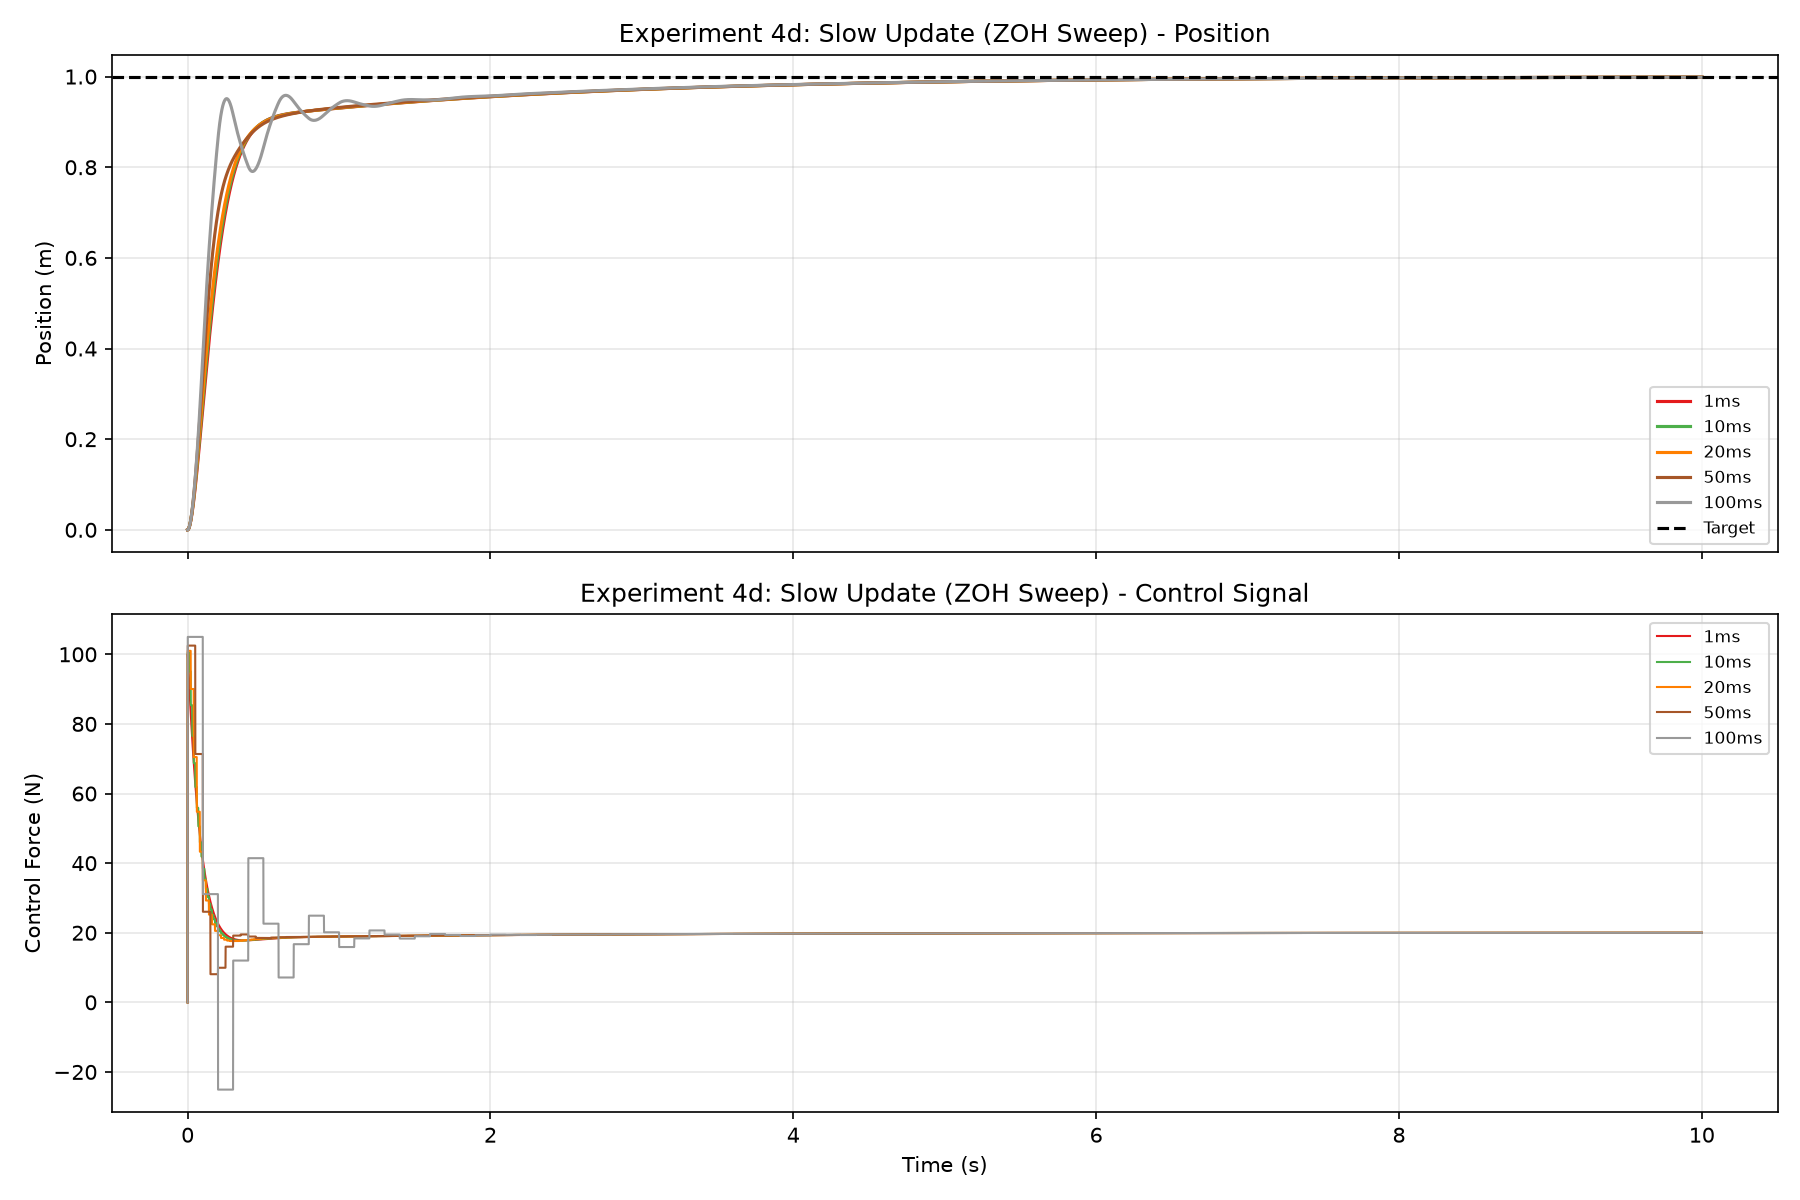
\includegraphics[width=0.9\linewidth]{experiment_plots/exp4d_zoh.png}
	\caption{Step responses for $T_s = 1, 10, 100, 200, 300$\,ms. Up to 100\,ms the curves are almost identical, then overshoot appears and at 300\,ms the output diverges.}
\end{figure}

\paragraph{The fix.}
Run the controller fast enough. The response is unchanged up to 100\,ms, and instability begins between 250\,ms and 300\,ms. A practical rule is to sample at least 10 times faster than the fastest closed-loop dynamics. Here the closed-loop time scale is a fraction of a second, so we recommend $T_s \le 10$\,ms (100\,Hz), which leaves a large safety margin.


\section{PID Tuning}


\section{Choosing the Gains}

Choosing $K_p$, $K_i$ and $K_d$ is called \emph{tuning}. The right method depends on what we know about the system.

\subsection{Two routes: with a model or on the hardware}

\paragraph{Route 1: tune on a model (simulation).}
If the system is simple enough that we can write down the equations that matter (as we did for the spring in Section~3), we build a simulation and test gains in it. It is fast, it cannot break anything, and it allows automatic search, for example a \textbf{grid search}: try every combination of gains from a list, simulate each one, compute the four measures of Section~4 and keep the best combination that satisfies our requirements (Section~8.3). Other search methods (random search, optimisation) work the same way.

\paragraph{Route 2: tune on the physical hardware.}
For a complex system (a drone in wind, a robot with many joints, a chemical process) an accurate model is very hard to build, and a simplified model may behave differently from the real machine. If the hardware is available and safe to test, we tune on it directly, using the hand-tuning procedure of Section~8.2 or the Ziegler--Nichols recipe of Section~8.4, which needs only experiments and no equations. In practice the two are combined: a model gives good starting gains and the final adjustment is made on the real machine.

\subsection{Manual tuning step by step}

First, what each gain does when it is \emph{increased} on its own (typical trends):

\begin{table}[h]
	\centering
	\small
	\begin{tabular}{@{}lllll@{}}
		\toprule
		Increase & Rise time & Overshoot & Settling time & Steady-state error \\
		\midrule
		$K_p$ & decreases & increases & small change & decreases (never zero alone) \\
		$K_i$ & decreases a little & increases & increases & removed \\
		$K_d$ & small change & decreases & decreases & no change \\
		\bottomrule
	\end{tabular}
	\caption{Effect of increasing each gain independently.}
\end{table}

The procedure (Figure~\ref{fig:tuning}):
\begin{enumerate}
	\item Set $K_i = K_d = 0$. Increase $K_p$ until the response is fast, accepting some overshoot and ringing.
	\item Increase $K_d$ until the bouncing is damped out.
	\item Increase $K_i$ slowly until the final offset disappears. Stop when overshoot or slow oscillation appears.
	\item Repeat steps 1--3 with small changes. If the force is jumpy, filter the derivative (Section~7b). If the actuator saturates, add anti-windup (Section~7a).
\end{enumerate}

\begin{figure}[h]
	\centering
	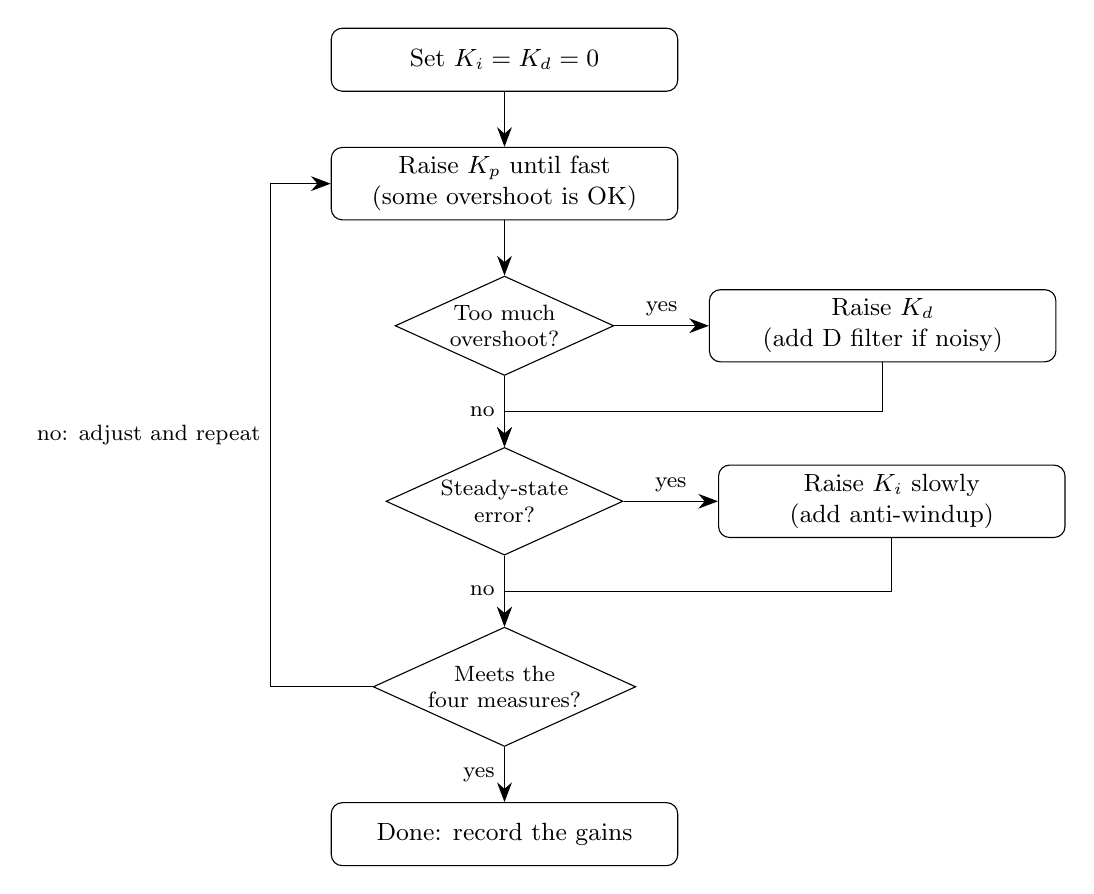
\begin{tikzpicture}[
		node distance=0.7cm,
		box/.style={draw, rectangle, rounded corners, align=center, minimum width=4.4cm, minimum height=0.8cm, font=\small},
		dec/.style={draw, diamond, aspect=2.2, align=center, inner sep=1pt, font=\footnotesize},
		>={Stealth[length=2.5mm]}
		]
		\node[box] (start) {Set $K_i = K_d = 0$};
		\node[box, below=of start] (kp) {Raise $K_p$ until fast\\(some overshoot is OK)};
		\node[dec, below=of kp] (os) {Too much\\overshoot?};
		\node[box, right=1.2cm of os] (kd) {Raise $K_d$\\(add D filter if noisy)};
		\node[dec, below=0.9cm of os] (sse) {Steady-state\\error?};
		\node[box, right=1.2cm of sse] (ki) {Raise $K_i$ slowly\\(add anti-windup)};
		\node[dec, below=0.9cm of sse] (ok) {Meets the\\four measures?};
		\node[box, below=0.7cm of ok] (done) {Done: record the gains};
		
		\draw[->] (start) -- (kp);
		\draw[->] (kp) -- (os);
		\draw[->] (os) -- node[above, font=\footnotesize] {yes} (kd);
		\draw[->] (os) -- node[left, font=\footnotesize] {no} (sse);
		\draw[->] (kd) |- ($(os.south)!0.5!(sse.north)$) -- (sse);
		\draw[->] (sse) -- node[above, font=\footnotesize] {yes} (ki);
		\draw[->] (sse) -- node[left, font=\footnotesize] {no} (ok);
		\draw[->] (ki) |- ($(sse.south)!0.5!(ok.north)$) -- (ok);
		\draw[->] (ok) -- node[left, font=\footnotesize] {yes} (done);
		\draw[->] (ok.west) -- ++(-1.3,0) |- node[pos=0.25, left, font=\footnotesize] {no: adjust and repeat} (kp.west);
	\end{tikzpicture}
	\caption{Manual tuning procedure.}
	\label{fig:tuning}
\end{figure}

\subsection{Model-based tuning: grid search on the test system}

On the spring system we searched $K_p \in \{20,40,60,100,150,200\}$, $K_i \in \{50,100,150,200,300,400\}$ and $K_d \in \{0,2,5,10,15,20\}$ (216 combinations), simulating each with the 30\,N force limit, anti-windup and derivative on the measurement (Section~7). A combination was accepted if the overshoot was at most 5\% and the final error was below 5\,mm, and among the accepted ones we chose the one with the shortest settling time (2\% band).

\begin{table}[h]
	\centering
	\begin{tabular}{@{}rrrrr@{}}
		\toprule
		$K_p$ & $K_i$ & $K_d$ & Overshoot (\%) & Settling time (s) \\
		\midrule
		100 & 400 & 5  & 0.8 & 0.62 \\
		150 & 400 & 15 & 1.3 & 0.67 \\
		60  & 200 & 2  & 0.0 & 0.68 \\
		\bottomrule
	\end{tabular}
	\caption{Three best combinations from the grid search (84 of 216 passed the filters).}
\end{table}

The best combination, $K_p=100$, $K_i=400$, $K_d=5$, settles in 0.62\,s, compared with 3.8\,s for the starting gains ($K_p=100$, $K_i=50$, $K_d=10$) of Section~6. The best $K_i$ lies at the edge of the searched range, so a wider range could do slightly better. A search is only as good as its constraints, so it is important to include the actuator limit: without the 30\,N clamp the best choice would use $K_p = 300$, which demands 300\,N at the first instant and is impossible on real hardware.

\subsection{Ziegler--Nichols on a second system}

Ziegler--Nichols (ZN) tunes a system without knowing its equations, using one experiment. We apply it to the second system
\begin{equation}
	G(s) = \frac{1}{(s+1)^3},
\end{equation}
which has no steady-state offset problem in the plant itself (DC gain 1) but is slow, because it contains three lags in series.

\paragraph{The recipe.}
\begin{enumerate}
	\item Use P control only ($K_i = K_d = 0$).
	\item Increase $K_p$ until the output oscillates steadily, neither growing nor dying out. This gain is the \textbf{ultimate gain} $K_u$ and the period of the oscillation is the \textbf{ultimate period} $T_u$.
	\item Take the gains from Table~\ref{tab:zn}.
\end{enumerate}

\begin{table}[h]
	\centering
	\begin{tabular}{@{}lccc@{}}
		\toprule
		Controller & $K_p$ & $T_i$ & $T_d$ \\
		\midrule
		P   & $0.5\,K_u$ & --- & --- \\
		PI  & $0.45\,K_u$ & $T_u/1.2$ & --- \\
		PID & $0.6\,K_u$ & $T_u/2$ & $T_u/8$ \\
		\bottomrule
	\end{tabular}
	\caption{Ziegler--Nichols table. The gains used by the code are $K_i = K_p/T_i$ and $K_d = K_p\,T_d$.}
	\label{tab:zn}
\end{table}

\paragraph{Finding $K_u$ and $T_u$.}
In simulation we raised $K_p$ and watched the output (Figure~\ref{fig:zn1}): at $K_p=7.5$ the oscillation dies out, at 8.5 it grows, and at about 8 it is steady. The calculation agrees. The closed loop has the characteristic equation $(s+1)^3 + K_p = s^3 + 3s^2 + 3s + (1+K_p) = 0$. It sits on the edge of stability when the product of the two middle coefficients equals the last one, $3\cdot 3 = 1 + K_p$, so
\begin{equation}
	K_u = 8, \qquad \omega_u = \sqrt{3}\ \text{rad/s}, \qquad T_u = \frac{2\pi}{\sqrt{3}} = 3.63\ \text{s}.
\end{equation}

\begin{figure}[h]
	\centering
	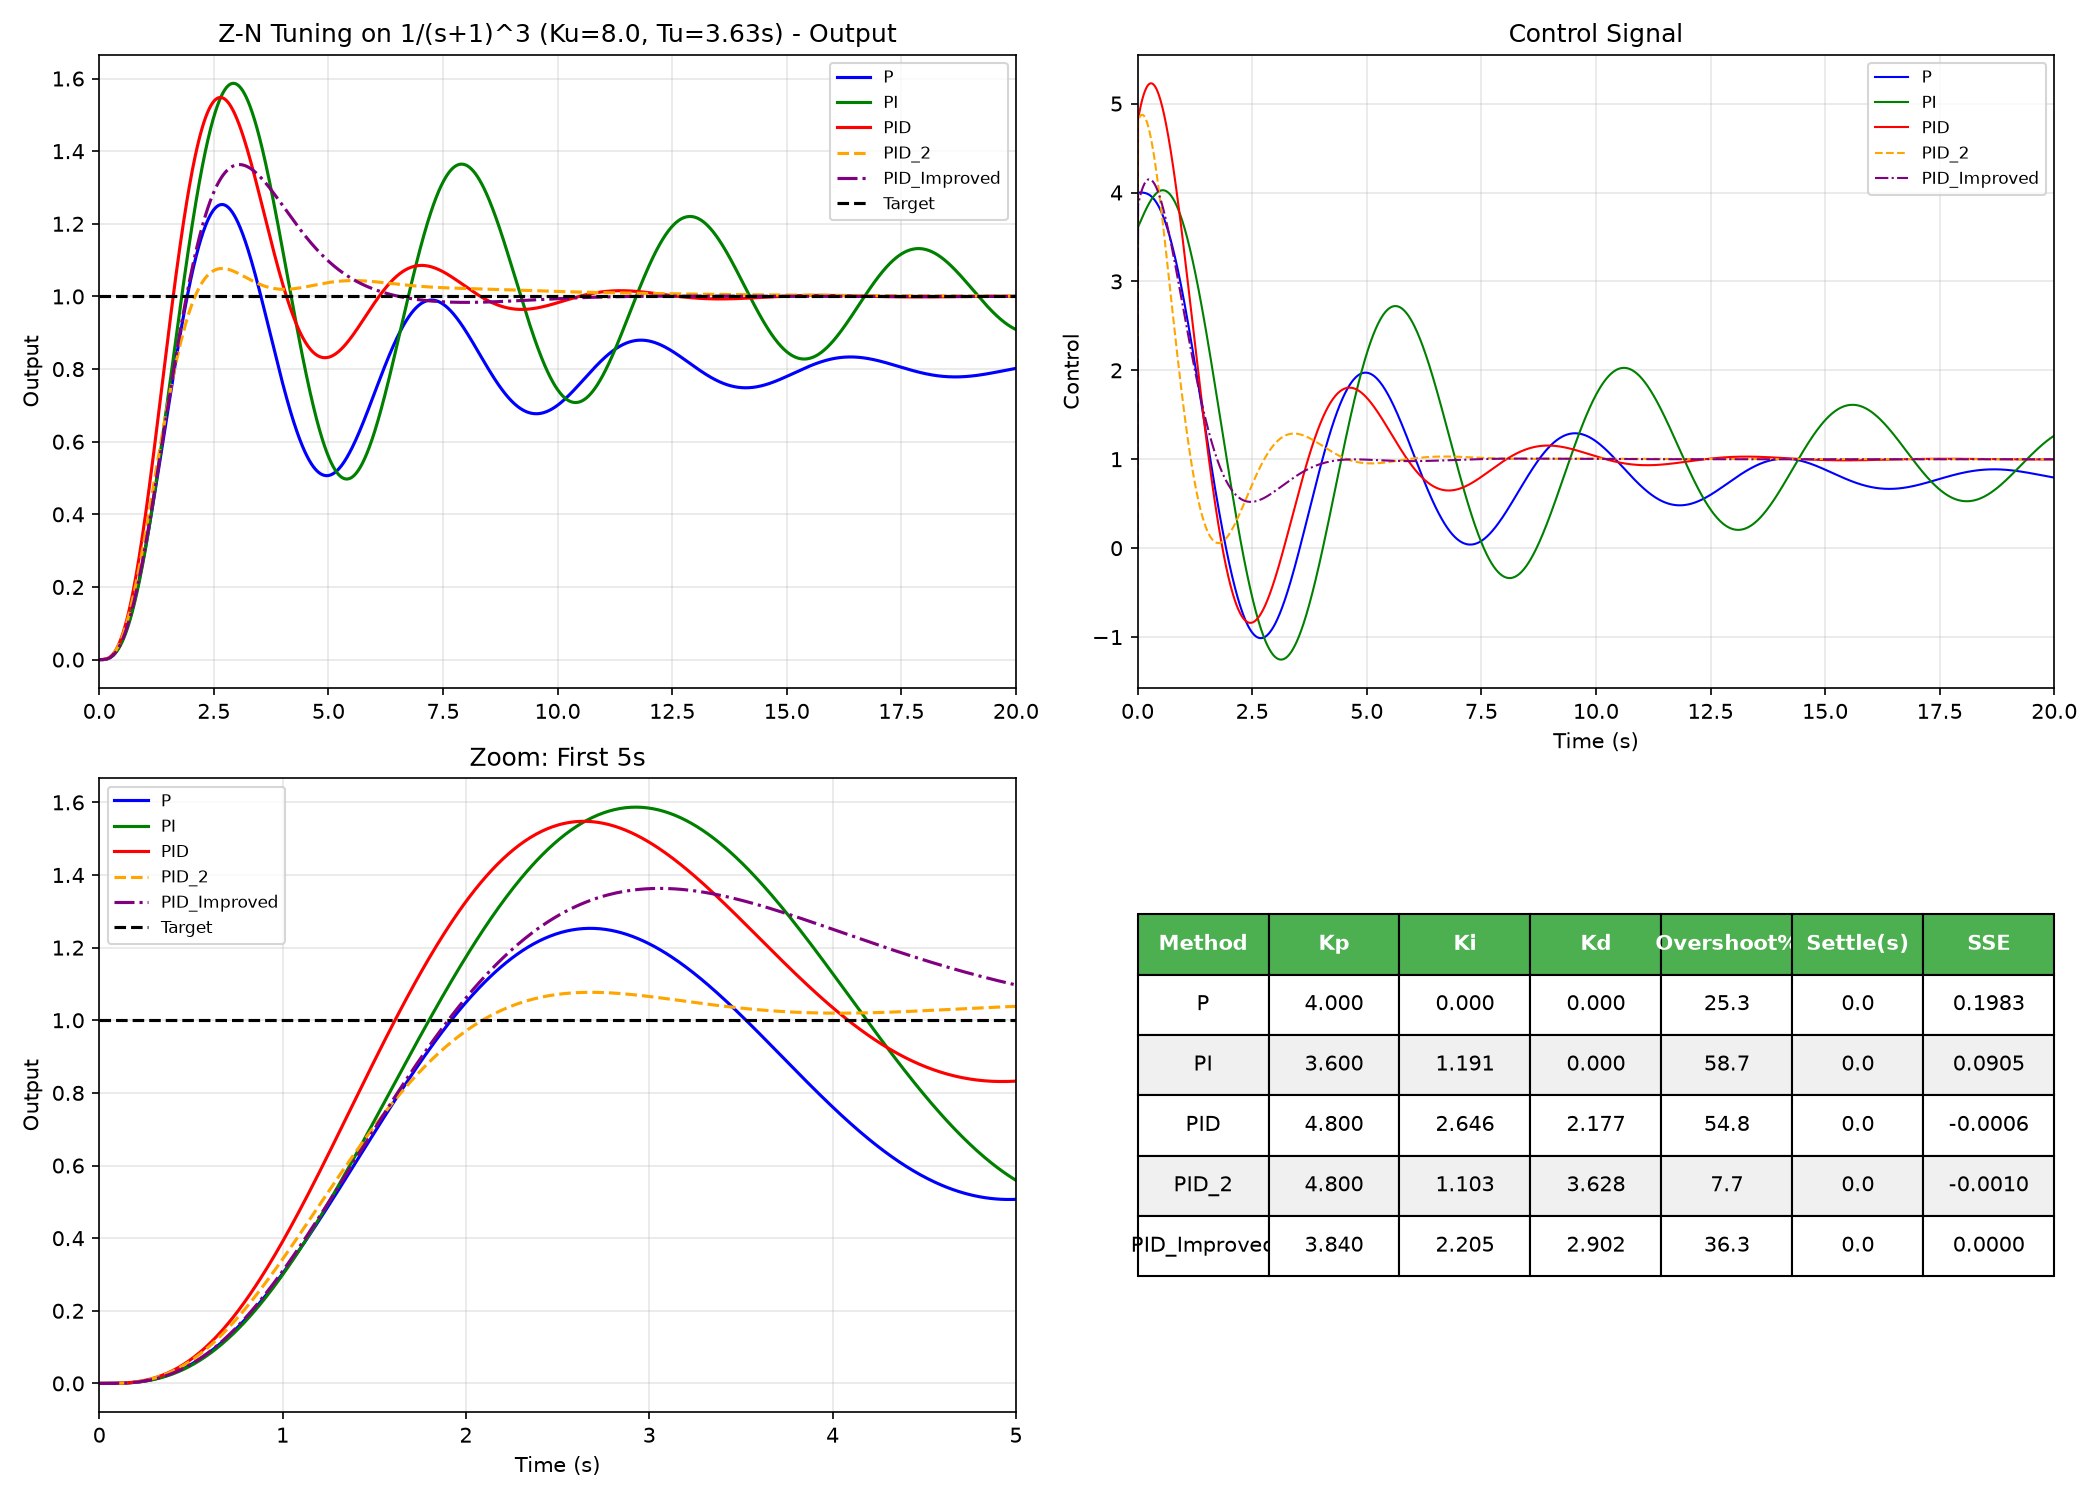
\includegraphics[width=0.85\linewidth]{experiment_plots/exp5_zn_tuning.png}
	\caption{P-only response of $1/(s+1)^3$ for $K_p = 7.5, 8, 8.5$: decaying, steady and growing oscillation. The steady one gives $K_u = 8$ and $T_u = 3.63$\,s.}
	\label{fig:zn1}
\end{figure}

\paragraph{Applying the table.}
\begin{table}[h]
	\centering
	\begin{tabular}{@{}lrrrrr@{}}
		\toprule
		Controller & $K_p$ & $K_i$ & $K_d$ & Overshoot (\%) & Settling time (s) \\
		\midrule
		ZN P   & 4.0 & --- & ---  & 23.4 & never ($e_{ss}=0.2$\,m) \\
		ZN PI  & 3.6 & 1.19 & ---  & 56.0 & 30.7 \\
		ZN PID & 4.8 & 2.65 & 2.18 & 52.4 & 9.89 \\
		\midrule
		Improved PID & 2.0 & 0.5 & 1.5 & 0.0 & 4.24 \\
		\bottomrule
	\end{tabular}
	\caption{Ziegler--Nichols gains and the improved hand-tuned result on $1/(s+1)^3$ (unit step, 2\% band).}
\end{table}

%\begin{figure}[h]
%	\centering
%	\includegraphics[width=0.85\linewidth]{fig_zn_result.png}
%	\caption{Step responses of $1/(s+1)^3$ with ZN P, PI, PID and the improved PID. ZN is fast but overshoots by more than 50\%.}
%\end{figure}

\paragraph{Improving it.}
ZN is designed for a fast reaction to disturbances and accepts a lot of overshoot, so its gains are only a starting point. We then followed the manual procedure of Section~8.2: we lowered $K_p$ from 4.8 to 2.0, which reduces the overshoot, and kept $K_d$ high relative to $K_p$ for damping. $K_i$ was lowered to 0.5 so that the integral does not overshoot the 1\,m target. The result is 0\% overshoot (down from 52.4\%) and a settling time of 4.24\,s (down from 9.89\,s).




\section{Code}
\section{Real robots and myths}
PID appears wherever a machine must hold a target despite disturbances. Table~\ref{tab:examples} lists five common examples.

\begin{table}[h]
	\centering
	\small
	% Set total width to text width. 
	% First three columns stay standard 'l', the last one (X) stretches and wraps.
	\begin{tabularx}{\textwidth}{XXXX}
		\toprule
		Application & Target / measured value & Controller output & How PID helps \\
		\midrule
		DC motor speed & Desired rpm; encoder measures actual rpm & Motor voltage (PWM duty) & P gives quick response, I removes the steady speed shortfall when the load changes, so speed stays constant under varying load. \\ \addlinespace
		Quadcopter drone & Desired roll, pitch, yaw angles; gyroscope measures them & Speed of each propeller & Separate PID loops for roll, pitch and yaw keep the drone level. D is important: it damps wobble caused by wind gusts. \\ \addlinespace
		Robot arm joint & Desired joint angle; encoder measures actual angle & Motor torque & The motor must hold the arm against gravity. \\ \addlinespace
		Line-following robot & Line centred under the sensor array; offset error & Difference in left/right wheel speeds & P steers back toward the line, D reduces zig-zagging at high speed. \\ \addlinespace
		Car cruise control & Desired speed; speedometer measures actual speed & Throttle position & I keeps the speed constant on a hill, where a constant extra force is needed. \\
		\bottomrule
	\end{tabularx}
	\caption{Real examples of PID control.}
	\label{tab:examples}
\end{table}

In every row the structure is the same as Figure~\ref{fig:general_control}: only the sensor, the actuator and the units of the gains change. Large systems such as drones and robot arms usually use \emph{several} PID loops at once, for example an outer loop that controls position and an inner loop that controls speed or torque.

\subsection{Common myths about PID}

\paragraph{Myth 1: ``Higher gains always give a better response.''}
\emph{Reality:} Increasing $K_p$ makes the response faster only up to a point. Beyond it the system overshoots, then oscillates, and with large enough gain becomes unstable (Section~8 finds this limit for the Ziegler--Nichols system). Good tuning is a trade-off between speed, overshoot and stability.

\paragraph{Myth 2: ``You always need all three terms.''}
\emph{Reality:} Many real controllers are only PI, because the D term amplifies sensor noise (Section~7b). Simple systems may even work with P alone if a small steady-state error is acceptable.

\paragraph{Myth 3: ``The integral term fixes everything.''}
\emph{Reality:} The I term removes steady-state error, but it adds lag and can cause overshoot. If the actuator saturates, the integral keeps accumulating (windup) and makes things worse unless anti-windup is added (Section~7a).

\paragraph{Myth 4: ``PID is the best controller for every problem.''}
\emph{Reality:} PID is popular because it is simple, cheap and works well for many single-input, single-output problems. For systems with several interacting variables, strict constraints or large delays, other methods such as LQR or model predictive control can perform better.

\paragraph{Myth 5: ``Once tuned, the gains are good forever.''}
\emph{Reality:} If the plant changes (a heavier payload, a worn motor, a different battery voltage), the best gains change too. Real systems often re-tune periodically or switch between stored sets of gains (gain scheduling).




\end{document}

